% -*- fill-column: 52 -*-
% (local-set-key (kbd "C-c C-f") 'display-fill-column-indicator-mode)

\chapter{Típusok és egyesítés}
Az első leckében megismertük a tényeket és
szabályokat, és kaptunk egy első képet arról, hogy
hogyan is néz ki egy Prolog program. A következőkben
azzal fogunk foglalkozni, hogy megvizsgáljuk az
alapvető alkotóelemeket, valamint a programok fő
mozgató rugóját, az \emph{egyesítést}.

A Prolog \emph{kifejezés}\/eknek négy típusa van:
atom, szám, változó vagy struktúra. Az egyes típusok
,,helyesírására'' más és más szabályok vonatkoznak
-- nézzük meg ezeket közelebbről!
\index{kifejezés}\index{tipus@típus}
\subsection*{Atomok}
Láttuk, hogy vannak ,,konkrét dolgok'', amelyeket
kisbetűvel í\-runk. Ezeket \emph{atom}\/oknak szokás
nevezni. Az atomok neve háromféleképpen képezhető:
\begin{enumerate}
\item Betűk, számok és az alsóvonás (\pr{\_})
  karakter kombinációja, de az első mindig egy
  kisbetű. Pl.: \pr{nil}, \pr{foo1}, \pr{bar\_42},
  \pr{baz\_\_}, \pr{ez\_1\_hosszú\_név}.
\item Különleges karakterek sorozata (ezekből lehet
  válogatni: \pr{\#\$\&*+-./:<=>?{@}\^{}\~{}}),
  pl.~\pr{.:.} vagy \pr{==>} vagy \pr{+}.
\item Aposztrófok közti karaktersorozat,
  pl. \pr{'Peti'} vagy \pr{'Abú Tálib'}.
\end{enumerate}
Az első fajtára már sok példát láttunk; a másodikról
majd később lesz szó; a harmadikat pedig jellemzően
akkor használjuk, ha nagybetűvel kezdődő vagy
szóközt tartalmazó nevet szeretnénk adni (ritka).

\begin{infobox}{}{foo--bar--baz}
A programozók előszeretettel használják a \pr{foo},
\pr{bar} és \pr{baz} neveket, amikor valamilyen
példát mutatnak, ahol maga a név nem
fontos. Hasonlóan, ha egy példában egy egész számot
kell választani, ez leggyakrabban a \pr{42} (a
\emph{Galaxis útikalauz stopposoknak} nyomán). Ilyen
és hasonló programozó-szubkultúrával kapcsolatos
érdekességekről rengeteget lehet olvasni a \emph{Zsargon
  fájl}\/ban,\footnote[2]{http://www.catb.org/jargon/html/}
nagyon szórakoztató olvasmány. (Sajnos csak angolul
hozzáférhető, de sokszor nem is igazán lehetne
lefordítani.)
\index{foo--bar--baz}
\index{zsargon fájl}
\end{infobox}

\subsection*{Számok}
A Prolog egész és valós számokat tud kezelni, a
megszokott jelölésekkel (de angol szokás szerint
a tizedesvessző helyett ponttal). A valós számoknál lehet
használni az ún.~\emph{exponenciális formát} is,
ahol egy \pr{e} betű után a 10 kitevője szerepel,
tehát pl.~ugyanazt a számot jelöli a \pr{1.23e5} és
\pr{123000.0}, vagy a \pr{4.56e-3} és \pr{0.00456}.
\index{exponenciális forma}

Egy egész és egy valós szám nem ugyanaz még akkor
sem, ha ugyanaz az értékük, tehát
\begin{query}
?- 1.23e5 = 123000.
\end{query}
értéke \pr{false}. Van viszont egy matematikai
egyenlőségvizsgálat (\pr{=:=}), és arra már
teljesül, hogy
\begin{query}
?- 1.23e5 =:= 123000.
\end{query}
(A számok közti műveletekről majd később lesz még
szó.)

\subsection*{Változók}
Ahogy láttuk, a ,,határozatlan dolgok''
(\emph{változók}) nagybetűvel vagy alsóvonással
kezdődnek, pl.~\pr{X}, \pr{\_}, \pr{\_Y}, \pr{\_z}.

Ezek közül a \pr{\_} változónév különleges: minden
alkalommal egy független változót jelöl. Tegyük fel
például, hogy egy sakkprogramban az állás
\begin{query}
tábla(világos, futó, c, 3).
\end{query}
alakú tényekkel van leírva. Ekkor világos összes
bábuját lekérdezhetjük úgy, hogy
\begin{query}
?- tábla(világos, X, _, _).
\end{query}
De ugyanez nem működne, ha más azonos változónevet
adnánk meg, pl.
\begin{query}
?- tábla(világos, X, _hely, _hely).
\end{query}

A többi változó egy-egy szabályon belül mindig
ugyanazt jelöli, de a szabályok közt már azok is
függetlenek, pl.~az alábbi programban az \pr{X} és
\pr{Z} a szabályok bal- és jobboldalán azonos
értéket kell, hogy felvegyen, de a két szabálynak
nincs hatása egymásra:
\begin{program}
ős(X, Z) :- szülő(X, Z).
ős(X, Z) :- szülő(X, Y), ős(Y, Z).
\end{program}

\subsection*{Összetett struktúrák}
A \emph{struktúra} értelmileg összetartozó dolgokat
kapcsol össze. Az alakja olyan, mint a tényeké: egy
névvel (atommal) kezdődik, ez a struktúra
\emph{funktora}, majd utána zárójelek közt,
vesszőkkel elválasztva a hozzátartozó további
,,dolgok'' -- ezek a struktúra \emph{paraméterei}, a
számuk pedig a funktor \emph{aritása}.
\index{struktúra}\index{funktor}\index{paraméter}
\index{aritás}
A paraméterek maguk is tetszőleges Prolog
kifejezések lehetnek, tehát atomok, számok, változók
vagy struktúrák.

Egy kétdimenziós pontot leírhatunk egy
\pr{pont(X,Y)} struktúrával. Ha ezután egy
háromszöget akarunk létrehozni, akkor azt 6
koordináta helyett leírhatjuk 3 ponttal:
\pr{háromszög(P1,P2,P3)} -- ez egy újabb
struktúra. Például
\begin{query}
?- P1 = pont(1,0), P2 = pont(0,2), P3 = pont(-1,0),
   T = háromszög(P1, P2, P3).
\end{query}
esetén a \pr{T} értéke
\begin{query}
háromszög(pont(1,0),pont(0,2),pont(-1,0))
\end{query}
lesz.

Lehetnek azonos névvel különböző aritású funktorok,
pl.~lehet készíteni egy 3D \pr{pont(X,Y,Z)} funktort
is. (Hasonlóan, az eltérő aritású tények/szabályok is
megférnek egymás mellett.)

\begin{infobox*}{}{Struktúra vagy tény?}
Fontos, hogy ne keverjük össze a tényeket és
struktúrákat. Alakra ugyanúgy néznek ki -- és
később látni fogjuk, hogy ez nem véletlen --, de
mást jelent a
\begin{verbatim}
gyártó(swift, suzuki).
\end{verbatim}
tény és az \pr{autó(swift,suzuki)} kifejezés. Az
előbbi kifejez egy kapcsolatot a modellnév és a
gyártó között, míg az utóbbi a két adatot egy
egységbe kapcsolja össze: az autó egy olyan dolog,
amihez tartozik egy modellnév és egy gyártó.
\end{infobox*}

\begin{problem}
Milyen típusúak (atom, szám, változó, struktúra) az
alábbi kifejezések? Vigyázat, van köztük olyan, ami
nem helyes Prolog kifejezés!
\begin{itemize}
\item \pr{Foo}
\item \pr{foo}
\item \pr{'Foo'}
\item \pr{\_foo}
\item \pr{'Foo bar baz'}
\item \pr{foo(bar, baz)}
\item \pr{42}
\item \pr{15(X, Y)}
\item \pr{+(bal, jobb)}
\item \pr{három(Kis(Cica))}
\end{itemize}
\end{problem}
\begin{problem}
Milyen struktúrával lehetne jól leírni egy
téglalapot? Egy négyzetet? Egy kört?
\end{problem}

\subsection*{Egyesítés}
Két kifejezés egyesíthető, ha azonosak, vagy ha a
bennük levő változókat be lehet úgy állítani, hogy
azonossá váljanak. Például a \pr{dátum(Év,Hónap,22)}
és a \pr{dátum(X,március,Y)} kifejezések
egyesíthetőek, ezt az \pr{=} segítségével tudjuk
ellenőrizni:\index{egyesítés}\index{\pr{=}}
\begin{query}
?- dátum(Év,Hónap,22) = dátum(X,március,Y).
Hónap = március,
X = Év,
Y = 22
\end{query}
(Mostantól az egyszerűség kedvéért a kérdésekre
kapott eredményeket egyszerűen a kérdés alá fogom
írni.)

Ugyanakkor pl.~a \pr{dátum(Év,Hónap,21)} és
\pr{dátum(X,Y,22)} kifejezések nem egyesíthetőek,
mivel a harmadik argumentum különböző; a
\pr{dátum(X,Y,Z)} és \pr{pont(X,Y,Z)} kifejezések
pedig azért nem, mert más a legkülső
(\emph{elsődleges}) funktoruk.
\index{funktor!elsődleges}

Visszatérve az első példára, az egyenlőség végtelen
sok más módon is kielégíthető, pl.
\begin{query}
Év = 1982,
Hónap = március,
X = 1982,
Y = 22
\end{query}
\dots de ezek kevésbé általánosak. Az egyesítés
mindig a legáltalánosabbat adja.

A pontos szabályok a következők:
\begin{enumerate}
\item Ha $S$ és $T$ \emph{konstansok} (tehát
  atomok vagy számok), akkor csak abban az esetben
  egyesíthetőek, ha azonosak.\index{konstans}
\item Ha $S$ változó, akkor a két kifejezés
  egyesíthető, és innentől kezdve $S$ ,,értéke''
  $T$ lesz. (Fordítva hasonlóan.)
\item Ha $S$ és $T$ is struktúrák, akkor pontosan akkor egyesíthetőek, ha
  \begin{itemize}
  \item megegyezik az elsődleges (legkülső) funktoruk
  \item ugyanannyi az aritásuk
  \item minden argumentumuk páronként egyesíthető
    (az ezekben szereplő változók ebben a rekurzív
    egyesítésben kaphatnak értéket)
  \end{itemize}
\end{enumerate}

Például a
\begin{query}
?- háromszög(pont(1,1),A,pont(2,3)) =
   háromszög(X,pont(4,Y),pont(2,Z)).
\end{query}
egyesítés az alábbi lépésekből áll:
\begin{enumerate}
\item Az elsődleges funktor (\pr{háromszög}) és az
  aritás (3) megegyezik.
\item \pr{pont(1,1) = X}
  (itt az \pr{X} megkapja a \pr{pont(1,1)} értéket)
\item \pr{A = pont(4,Y)}
  (itt az \pr{A} megkapja a \pr{pont(4,Y)} értéket)
\item \pr{pont(2,3) = pont(2,Z)}
  \begin{enumerate}
    \item Az elsődleges funktor (\pr{pont}) és az
      aritás (2) megegyezik.
    \item \pr{2 = 2}
    \item \pr{3 = Z}
      (itt a \pr{Z} megkapja a \pr{3} értéket)
  \end{enumerate}
\end{enumerate}

\subsection*{Egyesítés tényekben}
	
Az egyesítést ki lehet használni egy tényen belül
is. Egy szakasz függőlegességét megadhatjuk így:
\begin{program}
függőleges(szakasz(pont(X,_),pont(X,_))).
\end{program}

Most feltehetünk mindenféle érdekes kérdést:
\begin{query}
?- függőleges(szakasz(pont(1,1),pont(1,2))).
true
?- függőleges(szakasz(pont(1,1),pont(2,Y))).
false
?- függőleges(szakasz(pont(1,1),pont(X,2))).
X = 1
?- függőleges(szakasz(pont(X,3),P)).
P = pont(X,_)
\end{query}
Az utolsónál a rendszer az érdektelen
$y$-koordinátára valójában egy (implementációtól
függő) automatikusan generált nevet fog adni a
\pr{\_} helyett, pl.~\pr{\_123}.

\begin{problem}
Definiáld szakaszokra a vízszintességet is, majd
döntsd el a segítségével, hogy van-e olyan szakasz,
ami egyszerre vízszintes és függőleges is!
\end{problem}
\begin{problem}
Egyesíthetőek-e az alábbi kifejezéspárok? Ha igen,
milyen értéke lesz a változóknak?
\begin{itemize}
\item \pr{pont(A,B) = pont(1,2)}
\item \pr{pont(A,B) = pont(X,Y,Z)}
\item \pr{plusz(2,2) = 4}
\item \pr{+(2,D) = +(E,2)}
\item \pr{háromszög(pont(-1,0),P2,P3) =}\\
  \pr{háromszög(P1,pont(1,0),(pont(0,Y))}
\end{itemize}
\end{problem}
\begin{problem}
Az előző feladat végén a háromszögek milyen
családját írtuk le?
\end{problem}
\begin{problem}
Készíts egy szabályt, ami eldönti, hogy egy téglalap
oldalai a tengelyekkel párhuzamosak-e!
\end{problem}

\section{Kétféle olvasat}
Egy \pr{P :- Q, R.} alakú szabályt kétféleképpen
lehet értelmezni:
\begin{enumerate}
\item Leíró (\emph{deklaratív}) olvasatok:
  \begin{itemize}
    \item \pr{P} igaz akkor, ha \pr{Q} és \pr{R} igaz.
    \item \pr{Q} és \pr{R}-ből következik \pr{P}.
  \end{itemize}
  \index{olvasat!deklaratív}
\item Működés szerinti (\emph{procedurális}) olvasatok:
  \begin{itemize}
    \item Ahhoz, hogy megoldjuk \pr{P}-t,
      \emph{először} megoldjuk \pr{Q}-t, és
      \emph{aztán} megoldjuk \pr{R}-et.
    \item Ahhoz, hogy kielégítsük \pr{P}-t,
      \emph{először} kielégítjük \pr{Q}-t és
      \emph{aztán} kielégítjük \pr{R}-et.
  \end{itemize}
  \index{olvasat!procedurális}
\end{enumerate}
A legfontosabb különbség az, hogy a procedurális
olvasatokban számít a kifejezések sorrendje.

\subsection*{Logikai vagy}
A deklaratív olvasat pusztán logika. A kifejezéseket
eddig mindig vesszővel (\pr{,}) kapcsoltuk össze,
ami logikai \emph{és}\/t jelent. A logikai
(megengedő) \emph{vagy}\/ot a pontosvessző (\pr{;})
jelöli. A vesszőnek van elsőbbsége, tehát a \pr{P :-
  Q, R; S, T.} kifejezést úgy értelmezzük, mintha
\pr{P :- (Q, R); (S, T).} lenne. (Az elsőbbségről
még később lesz szó bővebben.)\index{\pr{;}}

A pontosvessző helyett mindig írhatunk külön
szabályokat, és fordítva, pl.~az
\begin{program}
ős(X, Z) :- szülő(X, Z).
ős(X, Z) :- szülő(X, Y), ős(Y, Z).
\end{program}
szabályt írhattuk volna egy sorban is:
\begin{program}
ős(X, Z) :- szülő(X, Z); szülő(X, Y), ős(Y, Z).
\end{program}
De általában a külön szabályokba írt változat jobban
olvasható.

\section{Nyomkövetés}
Ahhoz, hogy jobban megértsük a procedurális
olvasatot, kövessük végig, hogy mit csinál a
rendszer egy egyszerű feladat megoldásakor! Legyen a
program a következő:
\begin{program}
nagy(medve).
nagy(elefánt).
kicsi(macska).
barna(medve).
fekete(macska).
szürke(elefánt).
sötét(Z) :- fekete(Z).
sötét(Z) :- barna(Z).
\end{program}

A kérdés pedig:
\begin{query}
?- sötét(X), nagy(X).
\end{query}
Tehát ,,Mi az ami sötét színű és nagy?''

A megoldáshoz vezető lépések:
\begin{enumerate}
\item A teljesítendő célok listája \pr{sötét(X),
  nagy(X)}.
\item Végigmegyünk a programon az elejétől kezdve,
  hogy találunk-e a \pr{sötét(X)}-el egyesíthető
  szabály-fejet (vagy tényt, hiszen a tények
  tulajdonképpen szabályok, amelyeknek a törzse
  \pr{true}). A 7-es sor az első ilyen. Az egyesítés
  miatt \pr{Z = X}, a \pr{sötét(X)}-et
  helyettesítjük a szabály törzsével, az új
  cél-lista \pr{fekete(X), nagy(X)}.
\item Végigmegyünk a programon az elejétől kezdve,
  hogy találunk-e a \pr{fekete(X)}-el egyesíthető
  szabály-fejet. Az 5-ös sor az első ilyen. Az
  egyesítés miatt \pr{X = macska}, és mivel az 5-ös
  sornak nincsen törzse, az új cél-lista
  \pr{nagy(macska)}.
\item Most a \pr{nagy(macska)}-val egyesíthető szabályt keresünk, de ilyen nincsen.
  \begin{itemize}
    \item Visszalépünk egyet, és az \pr{X} változót
      ismét szabaddá tesszük. Keresünk egy újabb
      egyezést a \pr{fekete(X)}-el, onnan, ahol
      legutóbb abbahagytuk (5-ös sor után), de ilyen
      sincsen.
    \item Visszalépünk még egyet, és újabb egyezést
      keresünk a \pr{sötét(X)}-el, onnan kezdve,
      ahol legutóbb abbahagytuk (7-es sor után). Az
      első ilyen a 8. sorban van. Az egyesítés miatt
      \pr{Z = X}, a \pr{sötét(X)}-et helyettesítjük
      a törzzsel, az új cél-lista tehát
      \pr{barna(X), nagy(X)}.
  \end{itemize}
\item A program elejétől keresünk a \pr{barna(X)}-el
  egyesíthető szabályt. A 4-es sor az első ilyen. Az
  egyesítés miatt \pr{X = medve}, és nincs törzs,
  tehát az új cél-lista \pr{nagy(medve)}.
\item A program elejétől keresünk a
  \pr{nagy(medve)}-vel egyesíthető szabályt. Rögtön
  az első sorban meg is találjuk; nincs törzse, és
  így a cél-listánk elfogyott, készen vagyunk! Az
  \pr{X} értéke tehát \pr{medve}.
\end{enumerate}

Bár nem része a szabványnak, a legtöbb Prolog
rendszer lehetővé teszi a program végigkövetését a
\pr{trace} és \pr{notrace} parancsok segítségével:
\begin{query}
?- trace, sötét(X), nagy(X), notrace.
\end{query}
\index{nyomkövetés}
\index{\pr{trace}}\index{\pr{notrace}}

Ez minden egyes lépést kiír; ezek a következő
típusúak lehetnek:
\begin{itemize}
\item [Call] Egy új cél keresése indul
\item [Redo] Újra próbálkozik egy másik egyesítéssel
\item [Fail] A cél kielégítése sikertelen
\item [Exit] A cél kielégítése sikeres
\end{itemize}

\begin{problem}
Írd újra az alábbi programot pontosvessző nélkül!
\begin{program}
kiolvas(Szám, Szó) :-
    Szám = 1, Szó = egy;
    Szám = 2, Szó = kettő;
    Szám = 3, Szó = három.
\end{program}
\end{problem}
\begin{problem}
Mit ad az
\begin{program}
f(1, egy).
f(s(1), kettő).
f(s(s(1)), három).
f(s(s(s(X))), N) :- f(X, N).
\end{program}       
program az alábbi kérdésekre?
\begin{query}
?- f(s(1), A).
?- f(s(s(1)), kettő).
?- f(s(s(s(s(s(s(1)))))), C).
?- f(D, három).
\end{query}
\end{problem}
\begin{problem}
Vezesd végig a
\begin{query}
?- nagy(X), sötét(X)
\end{query}
kérdés megoldását!
\end{problem}
\begin{problem}
A \pr{trace}-t be lehet tenni egy szabály törzsébe
is, és akkor onnantól kapcsolódik be a
nyomkövetés. Írd át a 7.~sort az alábbira:
\begin{program}
sötét(Z) :- trace, fekete(Z).
\end{program}
Ezután nézd meg a
\begin{query}
?- sötét(X), nagy(X).
\end{query}
kérdést! Amikor belép a nyomkövetésbe, hagyd
továbbmenni -- mi történik? Mi a helyzet akkor, ha a
8.~sorhoz is hozzáadod a \pr{trace}-t, és újra
kipróbálod?
\end{problem}

\subsection*{A sorrend fontossága}

Ha nem vigyázunk, könnyen írhatunk végtelen rekurziót. Ez a legtisztább formájában úgy néz ki, hogy
\begin{program}
p :- p.
\end{program}

Ha most kiértékeljük a
\begin{query}
?- p.
\end{query}
kérdést, akkor a gép csak dolgozik és dolgozik, és
nem áll le. (Implementációtól függően ilyenkor vagy
van egy ,,Abort'' gomb, vagy a Ctrl-C
billentyűkombináció megnyomásával lehet a programot
leállítani.) Bonyolultabb esetekben előfordulhat,
hogy egy idő után valami olyan hibaüzenetet kapunk,
hogy ,,stack limit exceeded'', ami lényegében azt
jelenti, hogy a rekurzió túl mély lett.

Az érdekes az, hogy egy program, ami deklaratív
olvasatban helyes, vezethet végtelen rekurzióra
(tehát a procedurális olvasat szerint hibás). Nézzük
meg megint az \pr{ős} szabályt!
\begin{program}
ős(X, Z) :- szülő(X, Z).
ős(X, Z) :- szülő(X, Y), ős(Y, Z).
\end{program}
Itt két sorrendről beszélhetünk: a szabályok
sorrendjéről, és a szabályon belüli kifejezések
sorrendjéről. Vizsgáljuk meg az összes verziót!
\begin{program}
% A múltkori családfa egy része
szülő(ámna, mohamed).
szülő(abdulla, mohamed).
szülő(mohamed, zajnab).
szülő(mohamed, fátima).
szülő(fátima, huszajn).

% Eredeti
ős1(X, Z) :- szülő(X, Z).
ős1(X, Z) :- szülő(X, Y), ős1(Y, Z).

% Szabályok felcserélve
ős2(X, Z) :- szülő(X, Y), ős2(Y, Z).
ős2(X, Z) :- szülő(X, Z).

% Kifejezések felcserélve
ős3(X, Z) :- szülő(X, Z).
ős3(X, Z) :- ős3(Y, Z), szülő(X, Y).

% Mindkettő felcserélve
ős4(X, Z) :- ős4(Y, Z), szülő(X, Y).
ős4(X, Z) :- szülő(X, Z).
\end{program}
A deklaratív olvasat a cserék során lényegesen nem
változik, az mindig jó lesz. Mi a helyzet a
procedurális olvasattal?

Az \pr{ős1} a már ismert verzió:
\begin{query}
?- trace, ős1(abdulla, fátima).
Call: ős1(abdulla, fátima)
  Call: szülő(abdulla, fátima)
  Fail: szülő(abdulla, fátima)
Redo: ős1(abdulla, fátima)
  Call: szülő(abdulla, Y)
  Exit: szülő(abdulla, mohamed)
  Call: ős1(mohamed, fátima)
    Call: szülő(mohamed, fátima)
    Exit: szülő(mohamed, fátima)
  Exit: ős1(mohamed, fátima)
Exit: ős1(abdulla, fátima)
true
\end{query}

Az \pr{ős2} esetében először mindig nem-szülő őst
próbál keresni:
\begin{query}
?- trace, ős2(abdulla, fátima).
Call: ős2(abdulla, fátima)
  Call: szülő(abdulla, Y1)
  Exit: szülő(abdulla, mohamed)
  Call: ős2(mohamed, fátima)
    Call: szülő(mohamed, Y2)
    Exit: szülő(mohamed, zajnab)
    Call: ős2(zajnab, fátima)
      Call: szülő(zajnab, Y3)
      Fail: szülő(zajnab, Y3)
    Redo: ős2(zajnab, fátima)
      Call: szülő(zajnab, fátima)
      Fail: szülő(zajnab, fátima)
    Fail: ős2(zajnab, fátima)
    Redo: szülő(mohamed, Y2)
    Exit: szülő(mohamed, fátima)
    Call: ős2(fátima, fátima)
      Call: szülő(fátima, Y3)
      Exit: szülő(fátima, huszajn)
      Call: ős2(huszajn, fátima)
        Call: szülő(huszajn, Y4)
        Fail: szülő(huszajn, Y4)
      Redo: ős2(huszajn, fátima)
        Call: szülő(huszajn, fátima)
        Fail: szülő(huszajn, fátima)
      Fail: ős2(huszajn, fátima)
    Redo: ős2(fátima, fátima)
      Call: szülő(fátima, fátima)
      Fail: szülő(fátima, fátima)
    Fail: ős2(fátima, fátima)
  Redo: ős2(mohamed, fátima)
    Call: szülő(mohamed, fátima)
    Exit: szülő(mohamed, fátima)
  Exit: ős2(mohamed, fátima)
Exit: ős2(abdulla, fátima)
true
\end{query}

Az \pr{ős3} a rekurzív szabálynál először az ősséget
ellenőrzi, csak aztán a szülőséget:
\begin{query}
?- trace, ős3(abdulla, fátima).
Call: ős3(abdulla, fátima)
  Call: szülő(abdulla, fátima)
  Fail: szülő(abdulla, fátima)
Redo: ős3(abdulla, fátima)
  Call: ős3(X, fátima)
    Call: szülő(X, fátima)
    Exit: szülő(mohamed, fátima)
  Exit: ős3(mohamed, fátima)
  Call: szülő(abdulla, mohamed)
  Exit: szülő(abdulla, mohamed)
Exit: ős3(abdulla, fátima)
true
\end{query}

Az \pr{ős4}-nél végtelen rekurzió jön létre:
\begin{query}
?- trace, ős4(abdulla, fátima).
Call: ős4(abdulla, fátima)
  Call: ős4(X1, fátima)
    Call: ős4(X2, fátima)
      Call: ős4(X3, fátima)
        Call: ős4(X4, fátima)
          ...
\end{query}

Egy jó ökölszabály, hogy érdemes az egyszerűbb
szabályokat előre tenni (\pr{ős1} és \pr{ős3}), és a
szabályokon belül is az egyszerűbb kifejezések
jöjjenek előbb (\pr{ős1}).

\begin{problem}
Menjetek végig a fenti nyomkövetéseken soronként (ha
esetleg megspóroltátok volna), és legyetek biztosak
benne, hogy minden világos!
\end{problem}
\begin{problem}
Az \pr{ős3} esetében, ha további megoldást kérünk
(ami itt az ,,Abdulla őse Fátimának'' állítás egy
másik bizonyítását jelentené), akkor megint végtelen
rekurzióba kerül a program. Miért?  Nézd meg
nyomkövetéssel!
\end{problem}
\section{Projekt: színes hatszögek}
Most már készen állunk arra, hogy egy kicsit
komolyabb feladatot is megnézzünk.

Az alábbi játékban az a cél, hogy a 7 színes
hatszöget úgy helyezzük el a képen látható
alakzatban, hogy mindig csak azonos színek
találkozzanak:
\begin{center}
  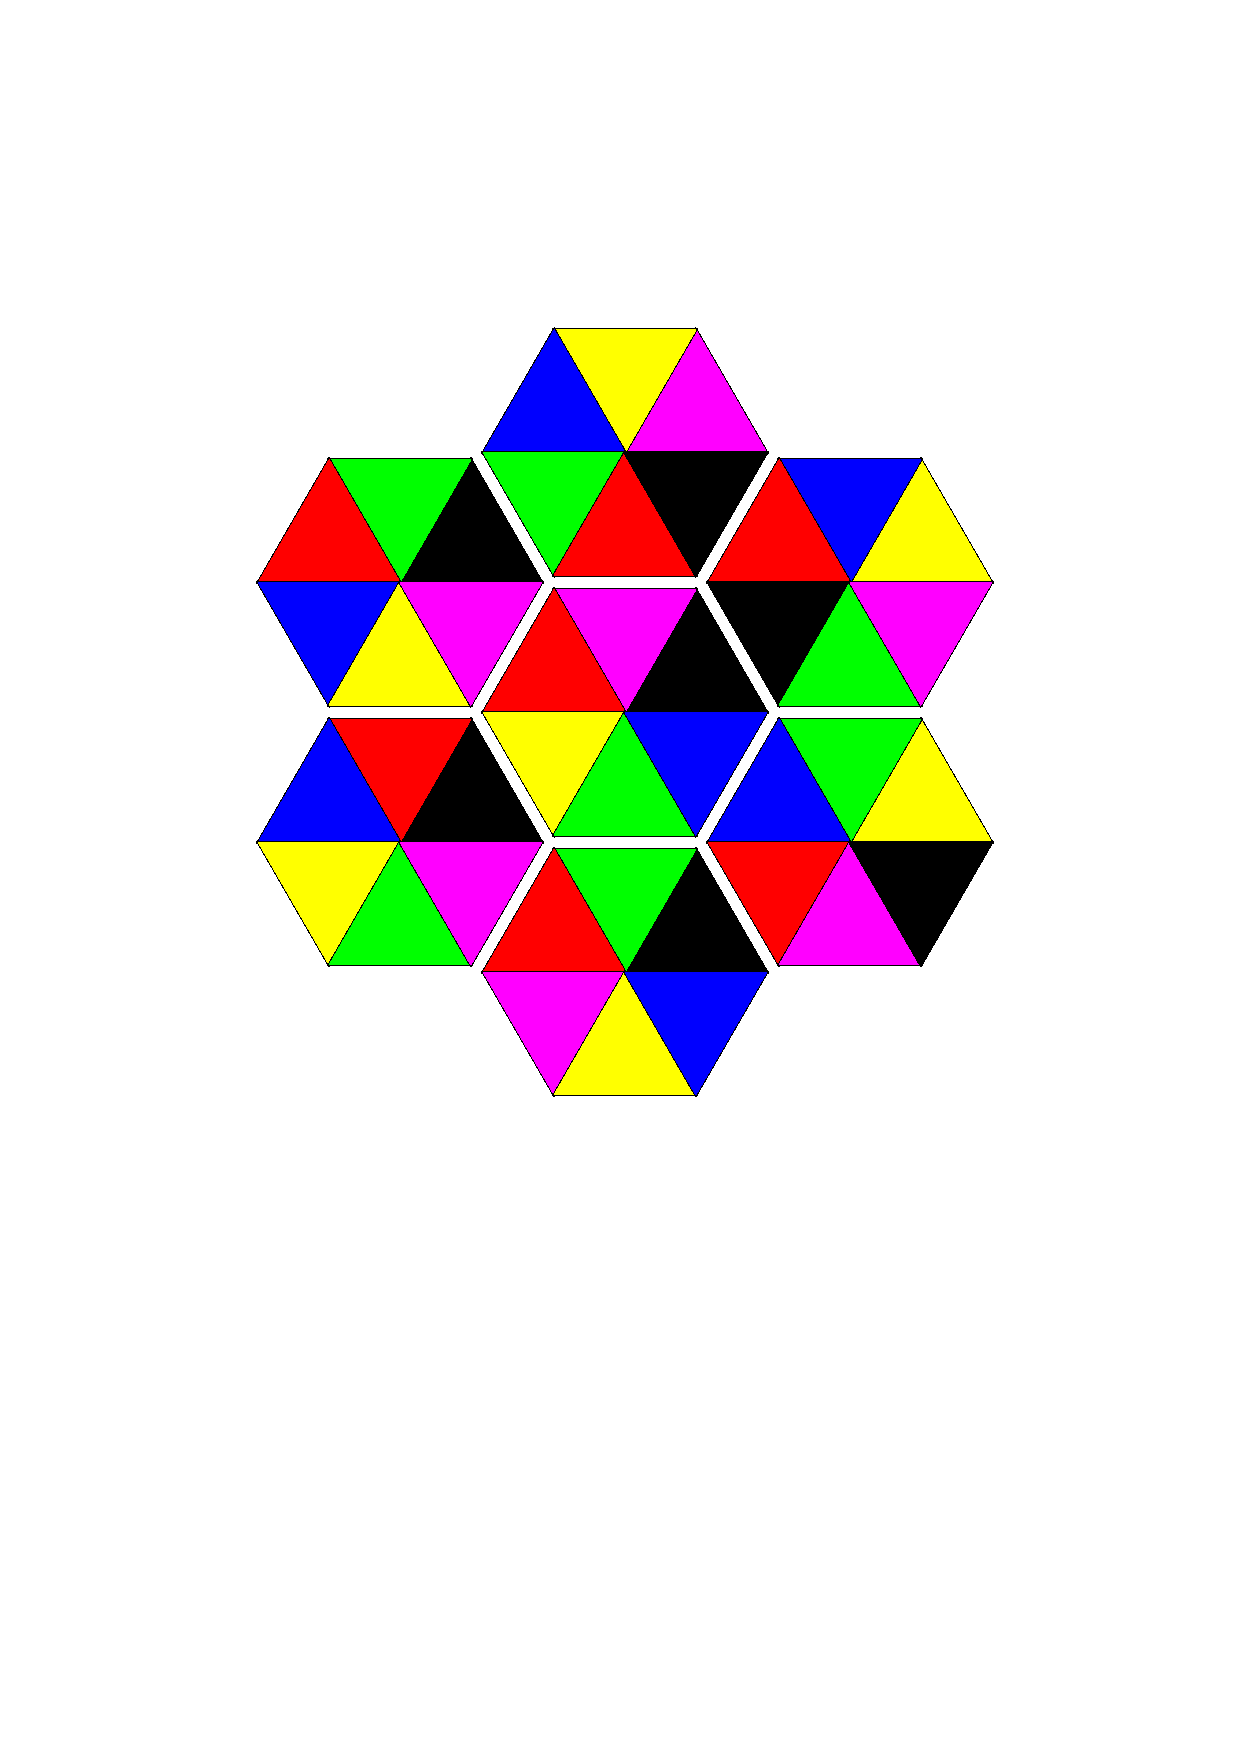
\includegraphics[width=.8\textwidth]{images/hexagons.pdf}
\end{center}

Ahhoz, hogy megoldjuk ezt a feladatot, először
valahogy le kell írnunk az ismert tényeket -- tehát
itt azt, hogy milyen lapok léteznek. A lapok színeit
egy \pr{l} struktúrába fogjuk össze, és a következő
tényeket kapjuk:
\begin{program}
lap(l(fekete,lila,sárga,kék,zöld,piros)).
lap(l(fekete,zöld,piros,kék,sárga,lila)).
lap(l(fekete,zöld,lila,sárga,kék,piros)).
lap(l(fekete,lila,piros,sárga,zöld,kék)).
lap(l(fekete,piros,kék,sárga,zöld,lila)).
lap(l(fekete,sárga,zöld,kék,piros,lila)).
lap(l(fekete,zöld,piros,lila,sárga,kék)).
\end{program}

Így például végig tudunk menni a lapokon a
\begin{query}
?- lap(L).
\end{query}
kérdés segítségével.

A lapok tetszőlegesen elforgathatóak, tehát a forgatásukra is kell valami mód. Ehhez először egyezzünk meg abban, hogy pontosan milyen elhelyezést jelent a színeknek egy sorrendje:
\begin{center}
  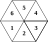
\includegraphics[width=.3\textwidth]{images/hexagon.pdf}
\end{center}

Tehát az első szín van délnyugatra, a második délre,
\dots a hatodik északnyugatra. Egy forgatás során
annyi történik, hogy valamelyik másik szín kerül
előre, de utána a sorrend változatlan. Ezt így
írhatjuk le:
\begin{program}
forgat(l(A,B,C,D,E,F), l(A,B,C,D,E,F)).
forgat(l(A,B,C,D,E,F), l(B,C,D,E,F,A)).
forgat(l(A,B,C,D,E,F), l(C,D,E,F,A,B)).
forgat(l(A,B,C,D,E,F), l(D,E,F,A,B,C)).
forgat(l(A,B,C,D,E,F), l(E,F,A,B,C,D)).
forgat(l(A,B,C,D,E,F), l(F,A,B,C,D,E)).
\end{program}

A következő feladat, hogy arra adjunk egy szabályt,
hogy mikor kapcsolódik helyesen két lap. Ehhez azt
is kell tudni, hogy egymáshoz képest hogyan
helyezkednek el. A \pr{kapcsolódik(L1, L2, Irány,
  F1, F2)} azt mondja, hogy ha az \pr{L1} laptól
\pr{Irány} irányba helyezzük le az \pr{L2} lapot,
akkor a két lap elforgatható egy \pr{F1} illetve
\pr{F2} helyzetbe úgy, hogy a találkozásuknál a
színek megegyeznek. Itt az irány leírására
használhatnánk a fent bevezetett számokat, de jobban
olvasható talán, ha égtájakat használunk. Nézzük meg
először a \pr{dny} (délnyugat) irányt!
\begin{program}
kapcsolódik(L1, L2, dny, F1, F2) :-
    forgat(L1, F1), forgat(L2, F2),
    F1 = l(X,_,_,_,_,_),
    F2 = l(_,_,_,X,_,_).
\end{program}
A törzs első sora csak annyit mond, hogy az \pr{F1}
és \pr{F2} az \pr{L1} és \pr{L2} elforgatottja; a
második és harmadik sor pedig azt biztosítja, hogy
az elforgatott lapokon a \emph{megfelelő} helyen
levő szín megegyezik (a többi nem számít). Mivel az
\pr{L1}-től délnyugatra van az \pr{L2}, ezért az
\pr{L1} délnyugati (első) színe az érdekes, az
\pr{L2}-nek pedig a szemben levő, tehát északkeleti
(negyedik) színe.

Teljesen hasonlóan felírhatjuk a többi égtájra is a
kapcsolódási szabályokat:
\begin{program}
kapcsolódik(L1, L2, d, F1, F2) :-
    forgat(L1, F1), forgat(L2, F2),
    F1 = l(_,X,_,_,_,_),
    F2 = l(_,_,_,_,X,_).
kapcsolódik(L1, L2, dk, F1, F2) :-
    forgat(L1, F1), forgat(L2, F2),
    F1 = l(_,_,X,_,_,_),
    F2 = l(_,_,_,_,_,X).
kapcsolódik(L1, L2, ék, F1, F2) :-
    forgat(L1, F1), forgat(L2, F2),
    F1 = l(_,_,_,X,_,_),
    F2 = l(X,_,_,_,_,_).
kapcsolódik(L1, L2, é, F1, F2) :-
    forgat(L1, F1), forgat(L2, F2),
    F1 = l(_,_,_,_,X,_),
    F2 = l(_,X,_,_,_,_).
kapcsolódik(L1, L2, ény, F1, F2) :-
    forgat(L1, F1), forgat(L2, F2),
    F1 = l(_,_,_,_,_,X),
    F2 = l(_,_,X,_,_,_).
\end{program}

Most már minden megvan ahhoz, hogy megkeressük a
megoldást. Ezt úgy találjuk meg, hogy veszünk 7
különböző (!) lapot, és felírjuk a rájuk vonatkozó
kapcsolódási feltételeket:
\begin{program}
megoldás(F1, F2, F3, F4, F5, F6, F7) :-
    lap(L1),
    lap(L2), L2 \= L1,
    lap(L3), L3 \= L1, L3 \= L2,
    lap(L4), L4 \= L1, L4 \= L2, L4 \= L3,
    lap(L5), L5 \= L1, L5 \= L2, L5 \= L3, L5 \= L4,
    lap(L6), L6 \= L1, L6 \= L2, L6 \= L3, L6 \= L4,
             L6 \= L5,
    lap(L7), L7 \= L1, L7 \= L2, L7 \= L3, L7 \= L4,
             L7 \= L5, L7 \= L6,
    kapcsolódik(L1, L2, dk,  F1, F2),
    kapcsolódik(F1, L7, ék,  F1, F7),
    kapcsolódik(F2, L3, ék,  F2, F3),
    kapcsolódik(F2, F7, é,   F2, F7),
    kapcsolódik(F3, L4, é,   F3, F4),
    kapcsolódik(F3, F7, ény, F3, F7),
    kapcsolódik(F4, L5, ény, F4, F5),
    kapcsolódik(F4, F7, dny, F4, F7),
    kapcsolódik(F5, L6, dny, F5, F6),
    kapcsolódik(F5, F7, d,   F5, F7),
    kapcsolódik(F6, F1, d,   F6, F1),
    kapcsolódik(F6, F7, dk,  F6, F7).
\end{program}
Itt a lapok számozása szintén a fenti módon
történik, a 7-es számú a középső lap. Az első hét
sor csak felveszi a lapokat, és biztosítja, hogy
mindegyik különböző legyen. Utána jönnek a szabályok
-- itt egy dologra kell figyelni, hogy (a
procedurális olvasat értelmében) a \pr{kapcsolódik}
szabályok kielégítése sorrendben történik, ezért
amint egy lapot ,,letettünk'', annak meghatározódik
a forgatása, tehát onnantól kezdve a forgatás
nélküli \pr{L} helyett az elforgatott \pr{F}-et kell
használni. Ezzel megköveteljük, hogy a
\pr{kapcsolódik}ban a ,,sima'' és ,,elforgatott''
változat megegyezzen, tehát ne tudja tovább forgatni
a lapot.

Keressük meg akkor a megoldást!
\begin{query}
?- megoldás(F1, F2, F3, F4, F5, F6, F7).
F1 = l(kék, zöld, piros, fekete, lila, sárga),
F2 = l(kék, sárga, lila, fekete, zöld, piros),
F3 = l(fekete, piros, kék, sárga, zöld, lila),
F4 = l(sárga, zöld, kék, piros, lila, fekete),
F5 = l(sárga, kék, fekete, zöld, piros, lila),
F6 = l(fekete, lila, piros, sárga, zöld, kék),
F7 = l(fekete, zöld, lila, sárga, kék, piros)
\end{query}

Ebben a programban rengeteg az ismétlés, ami nem túl
szép, de a jelenlegi eszközeinkből ennyire
futja. Nemsokára megismerkedünk a listákkal és a
számolással, amelyek segítségével a \pr{forgat} és a
\pr{kapcsolódik} szabályokat egy--egy sorban meg
lehetne oldani, és a \emph{megoldás}ban a lapok
különbözőségét is könnyebben lehetne biztosítani.
